\title{CS534 Implementation Assignment 3:\\Bagging and AdaBoost}
\author{
        Amit Bawaskar, Michael Lam\\
        EECS, Oregon State University\\
        %\email{}
        %\and
}

\documentclass[12pt]{article}
\usepackage[english]{babel}
\usepackage{graphicx}
\usepackage{subfig}
\usepackage{amsmath}
\usepackage{hyperref}
\hypersetup{
    colorlinks,%
    citecolor=green,%
    filecolor=magenta,%
    linkcolor=red,%
    urlcolor=cyan
}

%\underset{x}{\operatorname{argmax}}
%\underset{x}{\operatorname{argmin}}
\DeclareMathOperator*{\argmin}{arg\,min}
\DeclareMathOperator*{\argmax}{arg\,max}

\begin{document}
\maketitle

\begin{abstract}
In this assignment we implemented and evaluated bagging and AdaBoost using the decision stump as the base learner.
\end{abstract}

% -------------------------------------------------
\section{Introduction}
Ensemble methods such as bagging and AdaBoost work by taking a base learner and generating a set (ensemble) of hypotheses by varying the training set. The final hypothesis for classification is a majority vote of these hypotheses. The decision stump is a suitable base learner for bagging and especially AdaBoost because it is a weak learner, meaning it classifies slightly better than random.

In this assignment we implemented the decision stump, bagging and AdaBoost. For each ensemble method we evaluated the training and test errors as a function of the ensemble size.

\section{Decision Stump}
The decision stump is a one level decision tree. In this assignment all features and labels are binary. Therefore the decision stump is a one level binary tree with a binary feature test at the root node connected to two leaf nodes each containing a label.

Learning is done by going through every feature in the training data and computing the maximum information gain (minimum entropy). Once the feature with the maximum information gain is determined, the two leaf nodes are given the label of the majority class from splitting the training data on that feature. Inference is done by simply testing the feature and assigning the label following the appropriate branch.

For AdaBoost, decision stump learning also accepts a distribution of the data as input. Therefore each training example is weighted differently based on the distribution, which affects the information gain computation and leaf node labels in every iteration of AdaBoost.

\section{Bagging}
Bootstrap aggregating (bagging) is a machine learning ensemble algorithm designed to improve the stability and accuracy of machine learning algorithms used in statistical classification and regression. It also reduces variance and helps to avoid over fitting.

Bagging uses different training sets to learn independent smaller hypotheses which are combined to form a final hypothesis for classification. To make a training set (a.k.a. bootstrap sample), we independently draw N random instances of the whole training set (size N) with replacement and use the newly generated training set to learn a hypothesis. (For large N, each bootstrap sample will contain approximately 63.2\% unique examples.) After repeating the bootstrapping procedure to form a set of hypotheses, we combine these different hypotheses by majority voting to produce the best final hypothesis for the training set and test the testing data using this hypothesis. Since the random samples of the training data will vary, the hypothesis that we generate will account for most of the variations in the training data and the final combining of the hypotheses will eventually reduce the variance of the classifier.

\section{AdaBoost}
Boosting is an ensemble method that considers errors from previous hypotheses to decide how to sample the training data for the next iteration. This is in contrast to bagging, which individual classifiers were independent. Boosting works when the base learner is weak learner, i.e. its classification accuracy is slightly better than random.

AdaBoost is a particular boosting algorithm that maintains and updates a distribution over the training data based on the hypothesis error at each iteration. Thus each training data point is given more or less weight according to the distribution \(D\). At each iteration \(t\) AdaBoost records the current hypothesis and a weight \(\alpha_t\) computed from the weighted error \(\epsilon_t\). The distribution \(D\) is updated using the computed \(\alpha_t\).

These equations are shown below, for \(m\) training examples \(x_i\) and their labels \(y_i\), distribution \(D_t(i)\) at time \(t\) for \(i\)th example, hypothesis \(h_t\) from weak base learner (i.e. decision stump) at time \(t\) and \(Z\) is a normalization factor to make \(D_{t+1}\) a distribution:

\begin{align}
 \epsilon_t = \sum_{i=1}^{m} D_t(i) I(y_i \neq h_t(x_i)) \\
 \alpha_t = \frac{1}{2} log\left(\frac{1-\epsilon_t}{\epsilon_t}\right) \\
 D_{t+1}(i) = \frac{ D_{t}(i)exp(-\alpha_t y_i h_t(x_i)) }{Z} & & \forall i = 1,...,m \\
\end{align}

The final hypothesis is just the sign of the weighted sum of each hypothesis and its corresponding weight \(\alpha\).

\section{Results}
For bagging, figure \ref{fig:bagging_trainerrors} plots the training errors versus the ensemble size, and figure \ref{fig:bagging_testerrors} plots the test errors versus the ensemble size. Both error plots are averaged over 5 runs. (Due to the stochastic nature, we picked the best plots.)

\begin{figure}[!t]
  \centering
  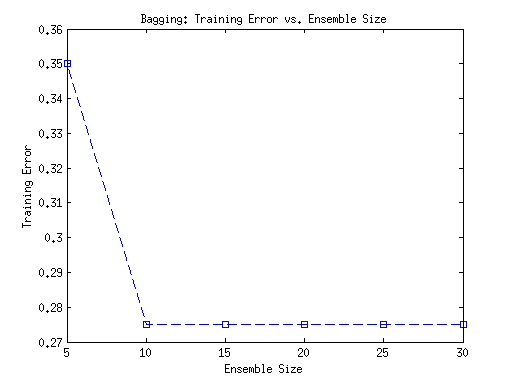
\includegraphics[scale=.6]{img/bagging_trainerrors.png}
  \caption{Bagging training errors on different ensemble sizes averaged over 5 runs.}
  \label{fig:bagging_trainerrors}
\end{figure}

\begin{figure}[!t]
  \centering
  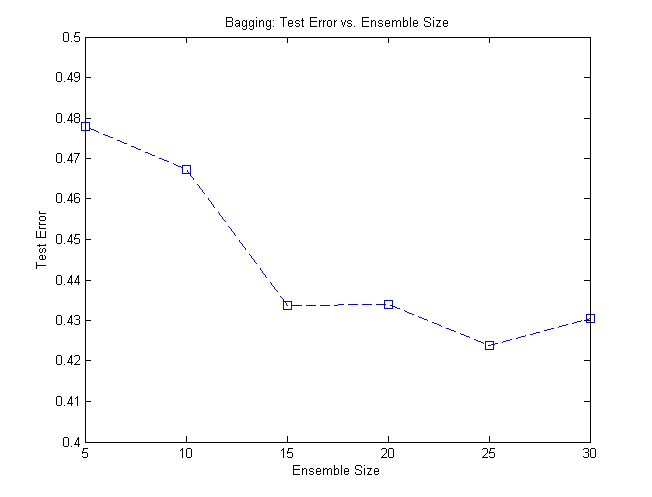
\includegraphics[scale=.6]{img/bagging_testerrors.png}
  \caption{Bagging test errors on different ensemble sizes averaged over 5 runs.}
  \label{fig:bagging_testerrors}
\end{figure}

For AdaBoost, figure \ref{fig:adaboost_trainerrors} plots the training errors versus the ensemble size, and figure \ref{fig:adaboost_testerrors} plots the test errors versus the ensemble size.

\begin{figure}[!t]
  \centering
  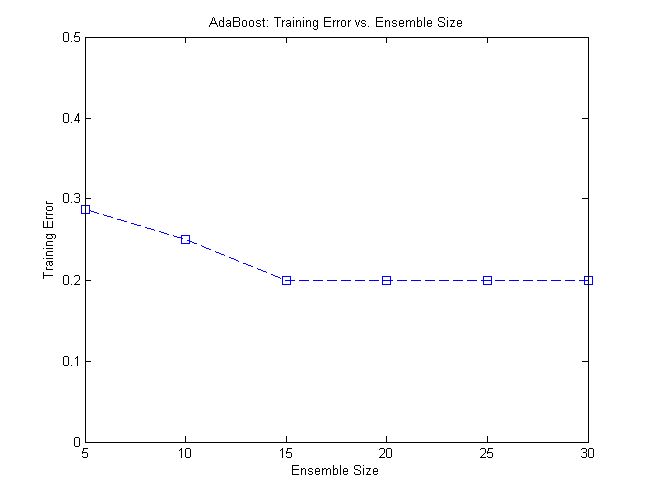
\includegraphics[scale=.6]{img/adaboost_trainerrors.png}
  \caption{AdaBoost training errors on different ensemble sizes.}
  \label{fig:adaboost_trainerrors}
\end{figure}

\begin{figure}[!t]
  \centering
  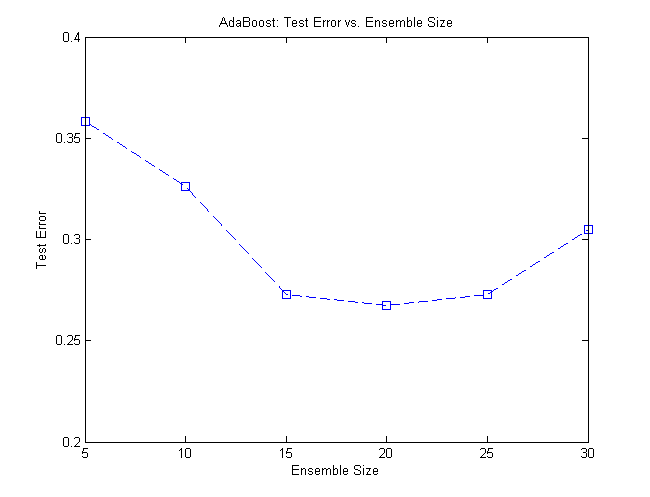
\includegraphics[scale=.6]{img/adaboost_testerrors.png}
  \caption{AdaBoost test errors on different ensemble sizes.}
  \label{fig:adaboost_testerrors}
\end{figure}

\section{Discussion}
For bagging the training error decreases as the ensemble size increases. Since the algorithm uses random sampling of the training data, it is expected that the more number of times we sample, the more we will tend to fit the training data. Hence, the training error decreases with increase in the ensemble size.

For the test/generalization error of bagging, the error decreases as we increase the number of ensembles. For a small ensemble size the algorithm has fewer samples to learn the hypothesis on and so makes more error on the test data. But as the size of the ensemble increases the errors reduce. It performs the best when the ensemble size is 25. After that, increasing the ensemble size does not help in reducing the error as we begin to overfit the hypothesis to the training data.

For AdaBoost, the training error appears to decrease as the ensemble size increases but then flattens out at ensemble size 15 and greater for the given training data. This indicates that while AdaBoost continues to select new hypotheses and weights (otherwise it would terminate), the training error does not improve. Interestingly, from observing the ensemble of hypotheses for ensemble size 30, there is a brief period after iteration 15 where the decision stump uses feature 17 iteration after iteration with more or less similar weights but with different leaf node labels. This may explain why the training error doesn't improve; the hypotheses and weights after iteration 15 have negligible impact on the final classifier.

The AdaBoost test/generalization error decreases and performs the best at around ensemble size 20, but then increases afterward. This trend is typical of test curves in machine learning; it indicates that test error decreases with the training error but eventually increases due to over fitting.

%\begin{align}
% 1+1=2
%\end{align}
%
%Figure \ref{fig:example} is an example.
%
%\begin{figure}[!t]
%  \centering
%  \includegraphics[scale=1]{img/example.png}
%  \caption{Caption example.}
%  \label{fig:example}
%\end{figure}

\end{document}
This is never printed
